\documentclass[12pt]{article}

% Packages
\usepackage{amsmath, amssymb, mathtools}
\usepackage{graphicx}
\usepackage{physics}
\usepackage{geometry}
\usepackage{enumitem}
\usepackage{bm}
\usepackage{listings}
\usepackage{xcolor}
\usepackage{float}

% Geometry settings
\geometry{letterpaper, margin=1in}
\setlength{\parindent}{0pt}

\definecolor{codegreen}{rgb}{0,0.6,0}
\definecolor{codegray}{rgb}{0.5,0.5,0.5}
\definecolor{codepurple}{rgb}{0.58,0,0.82}
\definecolor{backcolour}{rgb}{0.95,0.95,0.92}

\lstdefinestyle{mystyle}{
    backgroundcolor=\color{backcolour},   
    commentstyle=\color{codegreen},
    keywordstyle=\color{magenta},
    numberstyle=\tiny\color{codegray},
    stringstyle=\color{codepurple},
    basicstyle=\ttfamily\footnotesize,
    breakatwhitespace=false,         
    breaklines=true,                 
    captionpos=b,                    
    keepspaces=true,                 
    numbers=left,                    
    numbersep=5pt,                  
    showspaces=false,                
    showstringspaces=false,
    showtabs=false,                  
    tabsize=2
}

\lstset{style=mystyle}

% Title
\title{ECE 148 Homework 5}
\author{Sanjot Bains}
\date{\today}

\begin{document}

\maketitle

\section*{Background}
The periodic signal $f(t)$ has a period $T = 1$ and is defined as:
\[ f(t) = \sum_{m=1}^{7} a_m \sin(m \omega_0 t) \]
where $\omega_0 = \frac{2\pi}{T}$ is the fundamental frequency, and the amplitudes of the harmonics are given by:
\[ a_m = [ \ 9 \ 5 \ 8 \ 7 \ 1 \ 8 \ 9 \ ]. \]

The function $f(t)$ is sampled at 32 uniform intervals over one period.
\[ f(n) = f\left(\frac{n}{32}\right) \] for $n = 0, 1, \dots, 31$.

\vspace{1cm}
\begin{lstlisting}[language=Octave, caption=MATLAB Script to Initialize the Function]
T = 1; % Period of the signal
w_0 = 2 * pi / T; % Fundamental frequency
a_m = [9 5 8 7 1 8 9]; % Amplitude of harmonics

f = @(t) a_m(1) * sin(1 * w_0 * t) + a_m(2) * sin(2 * w_0 * t) + ...
         a_m(3) * sin(3 * w_0 * t) + a_m(4) * sin(4 * w_0 * t) + ...
         a_m(5) * sin(5 * w_0 * t) + a_m(6) * sin(6 * w_0 * t) + ...
         a_m(7) * sin(7 * w_0 * t);

% We will plot the function f(t) over one period.
t = linspace(0, T, 1000); % Time vector 
f_t = f(t); % Function values 

% We then take 32 uniform samples of the function f(t) over one period:
delta_T = T / 32; % Sampling interval
t_samples = 0:delta_T:(T-delta_T); % Sampled time vector
f_n = f(t_samples); % Sampled function values {f(n = 0, 1, ..., 31)}
\end{lstlisting}

\newpage
\section*{Problem 1: Time Function and Sampling}
The function $f(t)$ is plotted over one period ($0 \leq t < T$), along with its sampled values $f(n)$ for $n = 0, 1, \dots, 31$.

\begin{figure}[H]
    \centering
    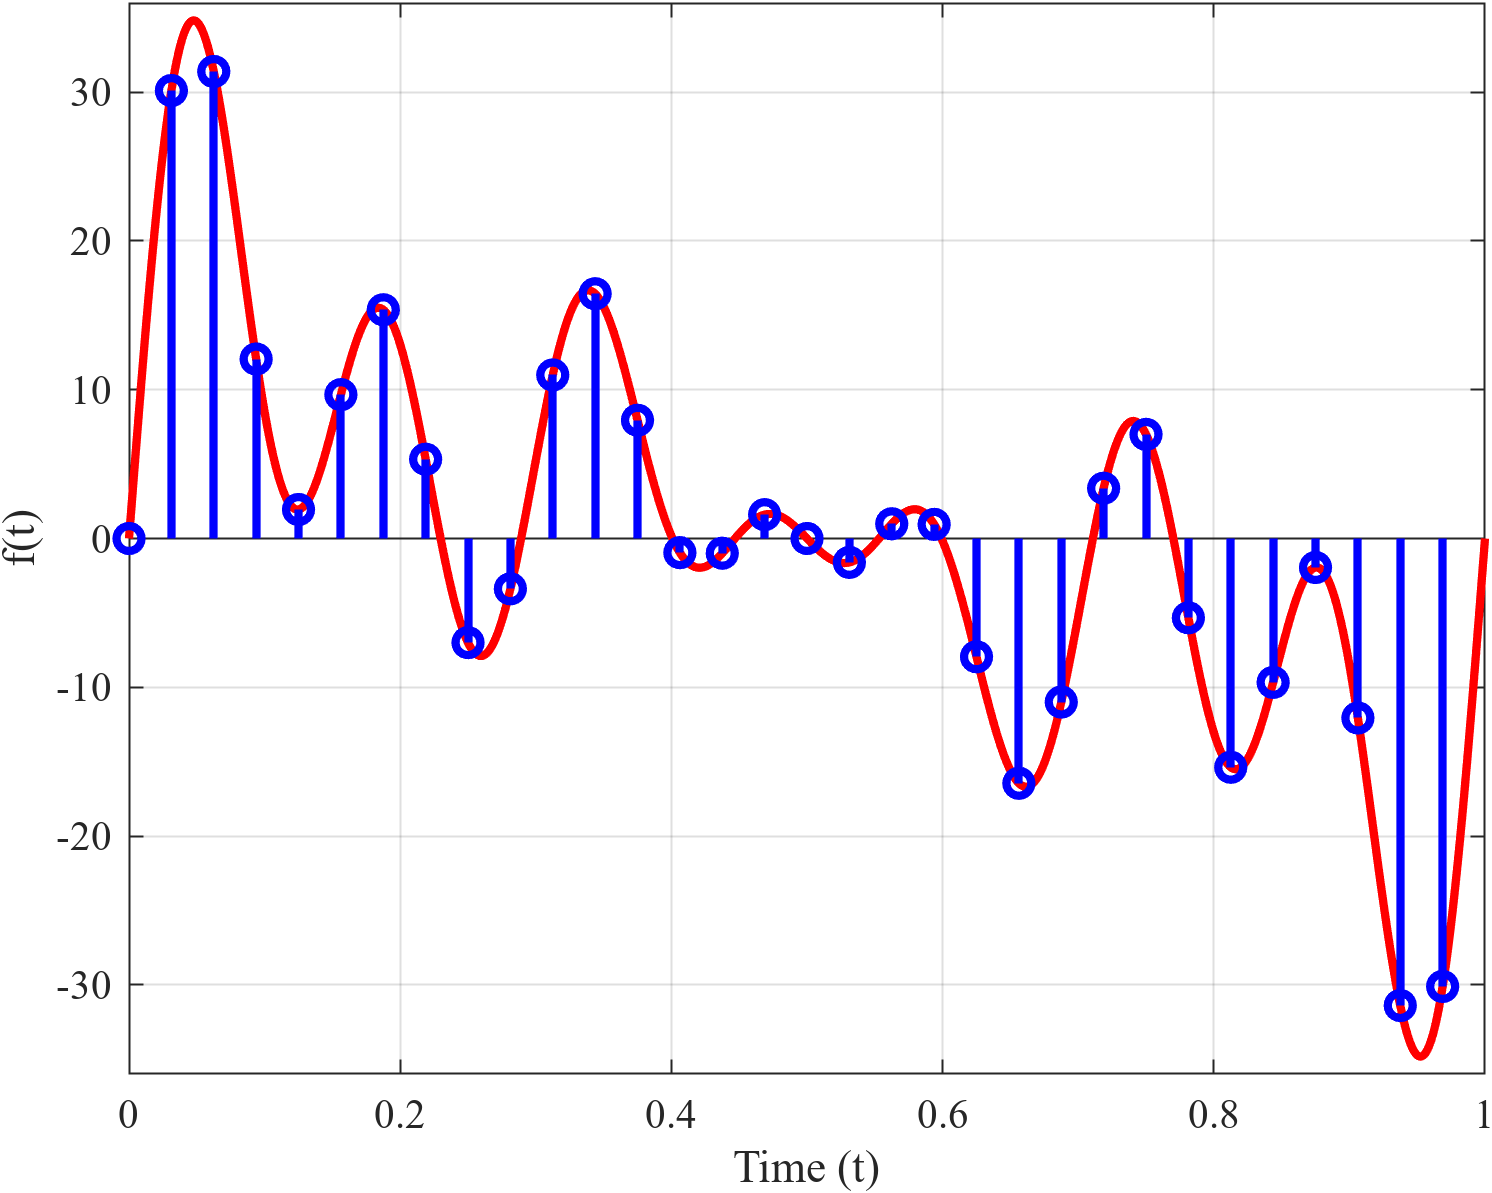
\includegraphics[width=0.8\textwidth]{f_t.png}
    \caption{Periodic Signal $f(t)$ and Sampled Values}
\end{figure}

\newpage
\section*{Problem 2: Fourier Series Expansion}
The periodic signal $f(t)$ is expressed in the form of a complex Fourier series expansion:
\[ F_m = \frac{1}{T} \int_{0}^{T} f(t) e^{-j m \omega_0 t} dt \]
where $m = -7, \dots, 7$ are the harmonic indices. The Fourier coefficients $F_m$ are computed numerically, and their magnitudes are plotted below:

\begin{figure}[H]
    \centering
    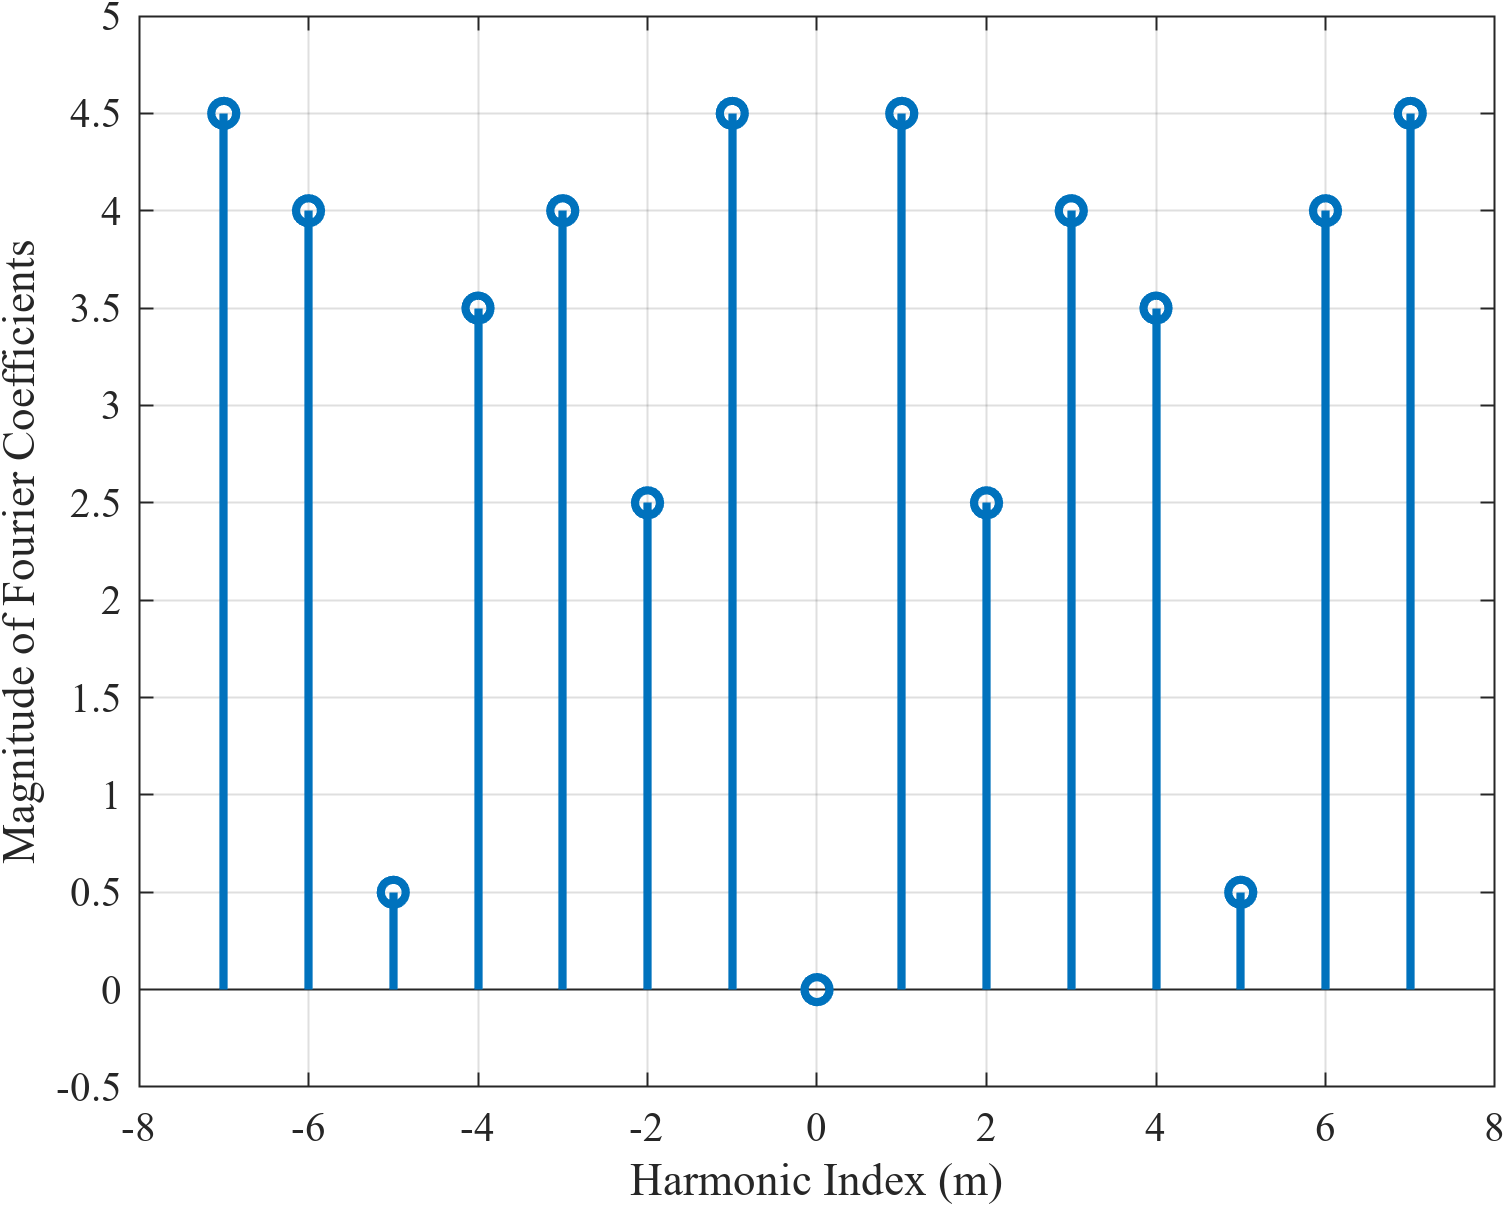
\includegraphics[width=0.8\textwidth]{F_m.png}
    \caption{Fourier Coefficients $F_m$}
\end{figure}

The Fourier coefficients are computed using the following MATLAB code:
\begin{lstlisting}[language=Octave, caption=MATLAB Script to Compute Fourier Coefficients]
N = 7;  % Number of harmonics to compute (from -N to N)
m = -N:N;  % Harmonic indices corresponding to F_m 
F_m = zeros(size(m));  % Complex Fourier coefficients (vector from -N to N) 
dt = t(2) - t(1);   % Calculate dt for numerical integration
    
% Calculate each coefficient using rectangular integration
for i = 1:length(m)
    integrand = f_t .* exp(-1j * m(i) * w_0 * t);
    F_m(i) = (1/T) * sum(integrand) * dt; 
end
clear i integrand;
\end{lstlisting}

The complex Fourier coeffiecients are:
\[ F_m = \begin{bmatrix}
    \ 0 + 4.5j \ \\
    \ 0 + 4j \ \\
    \ 0 + 0.5j \ \\
    \ 0 + 3.5j \ \\
    \ 0 + 4j \ \\
    \ 0 + 2.5j \ \\
    \ 0 + 4.5j \ \\
    \ 0 + 0j \ \\
    \ 0 - 4.5j \ \\
    \ 0 - 2.5j \ \\
    \ 0 - 4j \ \\
    \ 0 - 3.5j \ \\
    \ 0 - 0.5j \ \\
    \ 0 - 4j \ \\
    \ 0 - 4.5j \ \\
    \end{bmatrix} \]
The physical frequencies corresponding to the Fourier coefficients are given by $f_m = m \omega_0 / (2\pi)$.
The physical frequencies are:
\[ F_m = \begin{bmatrix}
    \ -7 \ \\
    \ -6 \ \\
    \ -5 \ \\
    \ -4 \ \\
    \ -3 \ \\
    \ -2 \ \\
    \ -1 \ \\
    \ 0 \ \\
    \ 1 \ \\
    \ 2 \ \\
    \ 3 \ \\
    \ 4 \ \\
    \ 5 \ \\
    \ 6 \ \\
    \ 7 \ \\
    \end{bmatrix} \text{Hz} \]


\newpage
\section*{Problem 3: Fourier Transform of Periodic Functions}
The Fourier transform $F(j\omega)$ of the periodic function $f(t)$ is determined and plotted. The amplitudes and physical frequencies of the peaks are identified.

\begin{figure}[H]
    \centering
    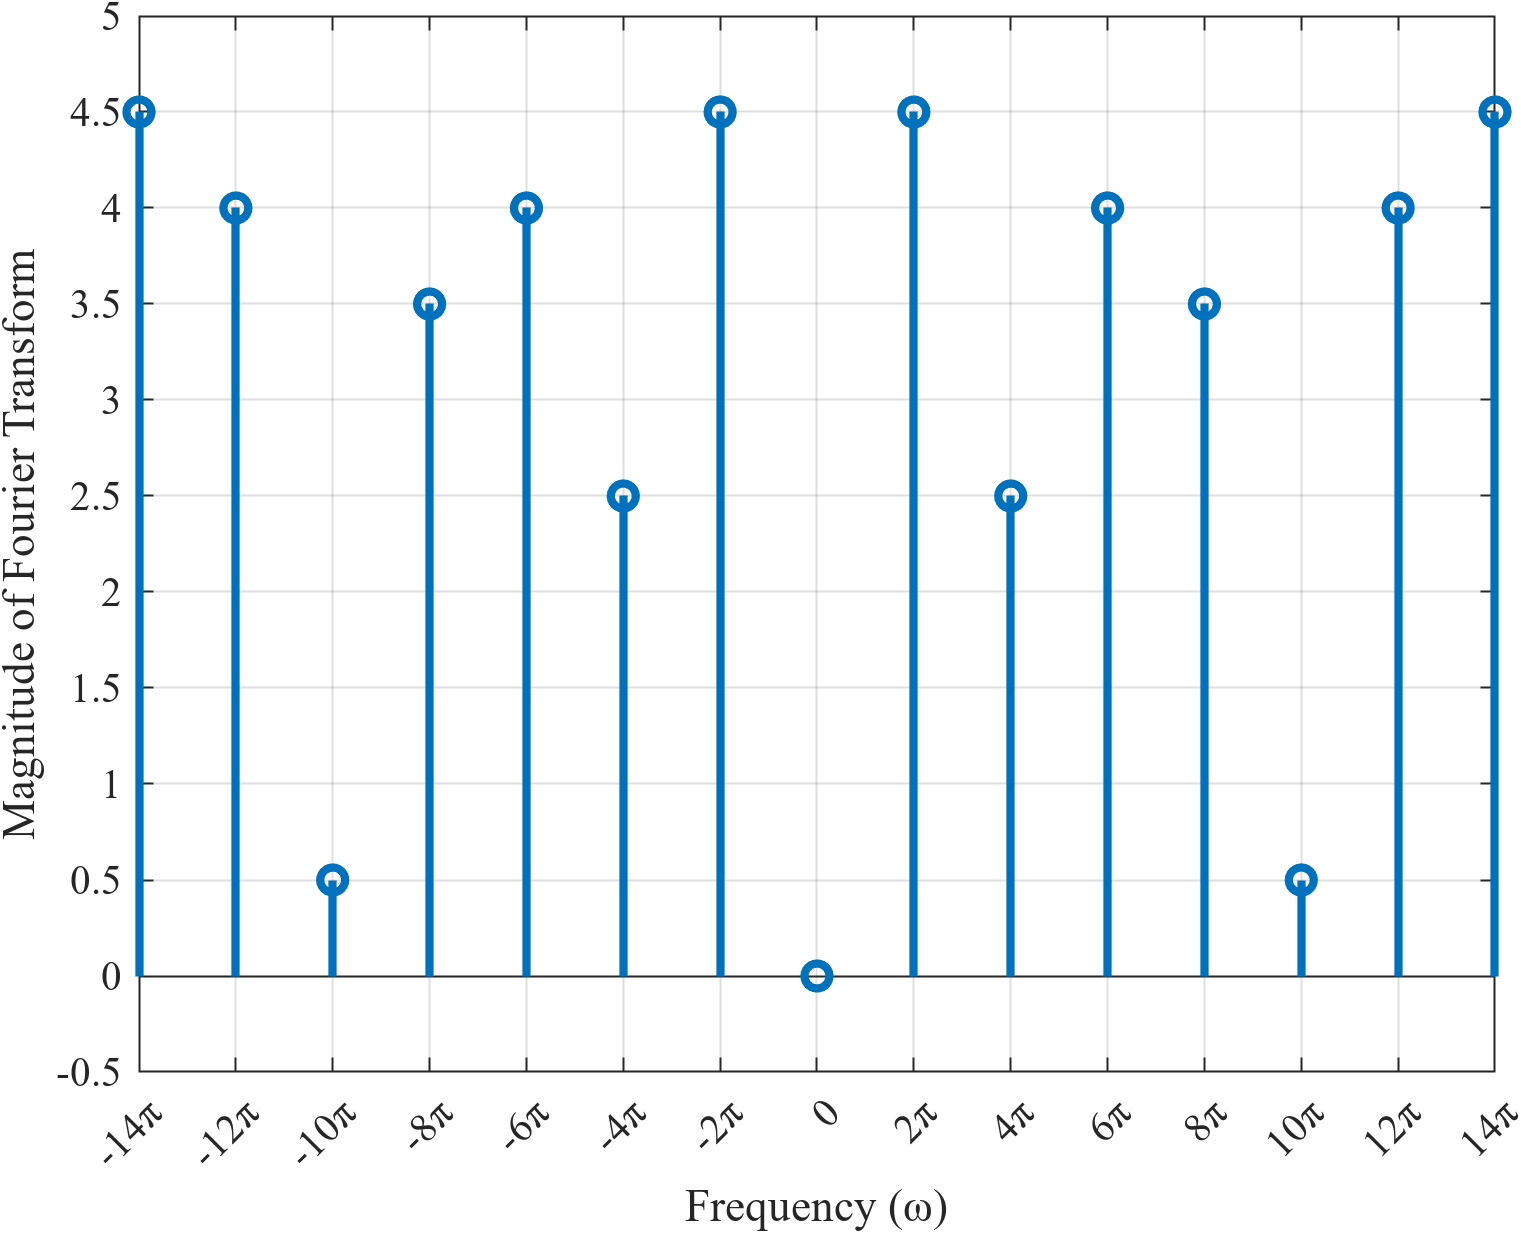
\includegraphics[width=0.8\textwidth]{F_j_omega.png}
    \caption{Fourier Transform $F(j\omega)$}
\end{figure}

The Fourier transform is formulated as following:
\[
F(j\omega) = \sum_{m=-7}^{7} F_m \delta(\omega - m \omega_0) \]
where $\delta(\cdot)$ is the Dirac delta function. 

\newpage
\section*{Problem 4: DTFT}
The Discrete-Time Fourier Transform (DTFT) $F(e^{j\Omega})$ of the 32-point time-domain sequence $f(n)$ is computed and plotted over the interval $(-\pi, \pi)$.

\begin{figure}[H]
    \centering
    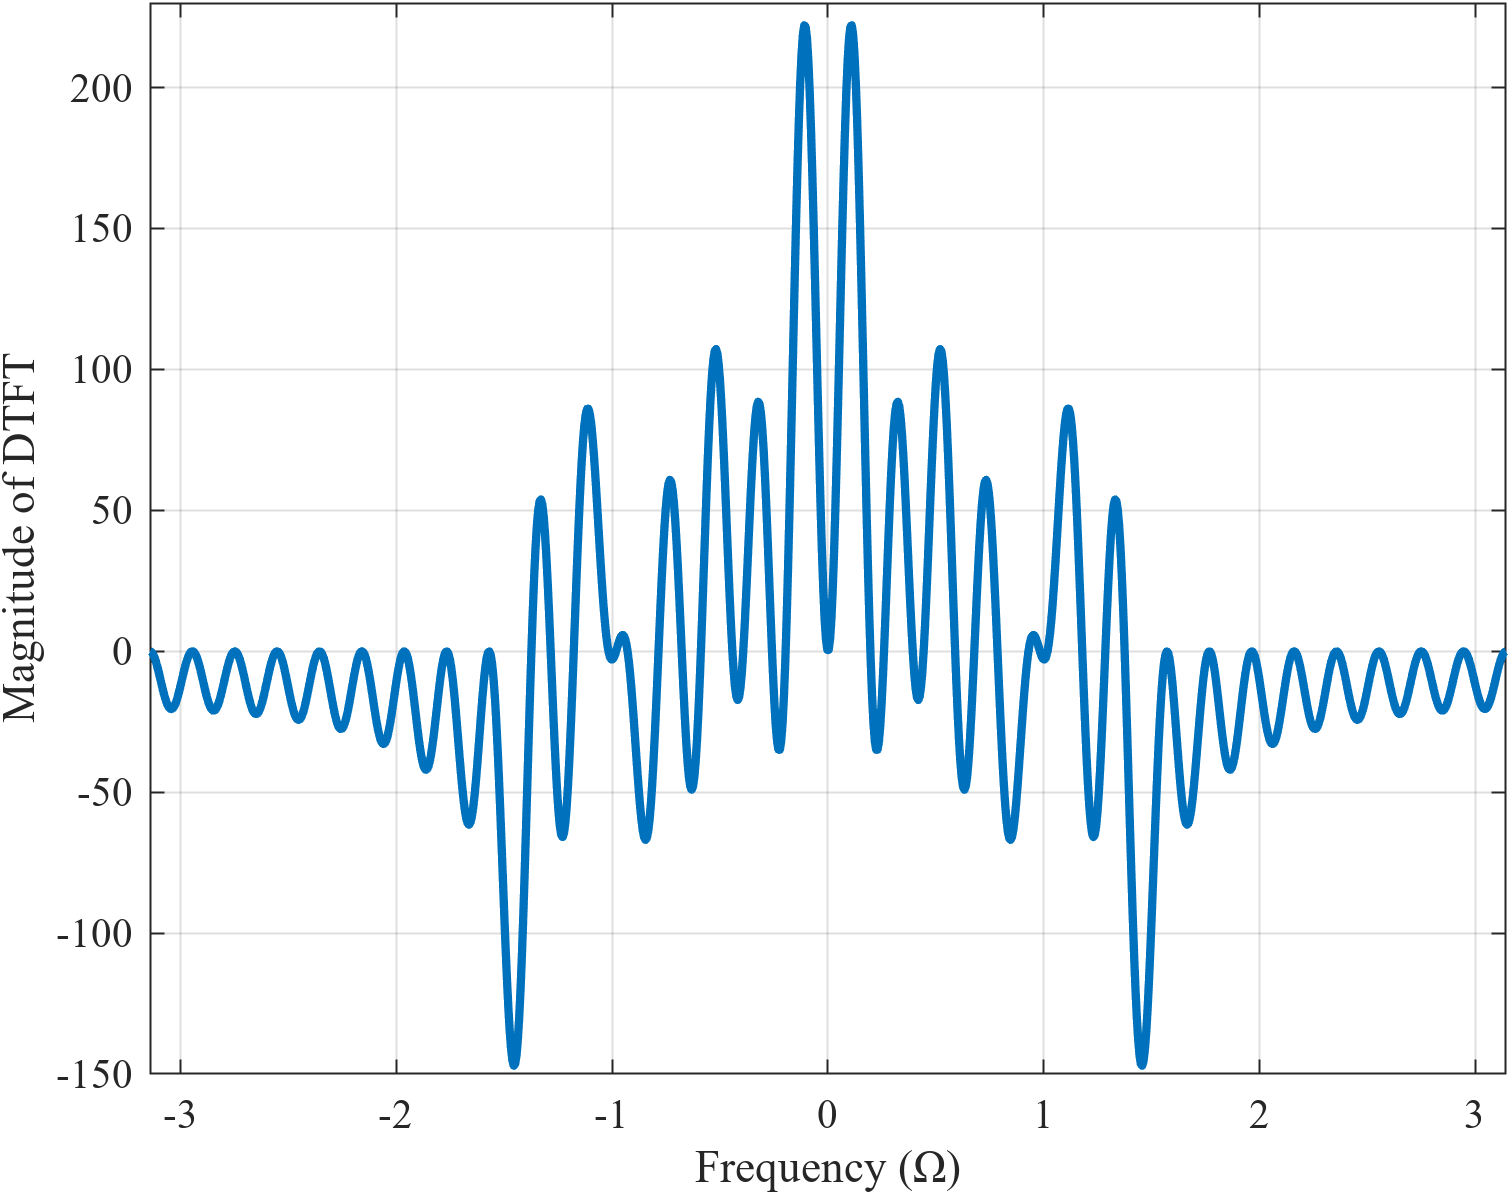
\includegraphics[width=0.8\textwidth]{F_Omega.png}
    \caption{DTFT $F(e^{j\Omega})$}
\end{figure}

\begin{lstlisting}[language=Octave, caption=MATLAB Script to Compute DTFT]
Omega = linspace(-pi, pi, 1000); % Frequency range 

F_Omega = zeros(size(Omega));
% Compute the DTFT using the Fourier coefficients
for n = 1:length(Omega)
    F_Omega(n) = sum(f_n .* exp(-1j * Omega(n) * (0:31)));
end
\end{lstlisting}


\newpage
\section*{Problem 5: DFT}
The 32-point DFT of the sampled sequence $f(n)$ is computed and plotted. The amplitudes and locations of the peaks are identified.

\begin{figure}[H]
    \centering
    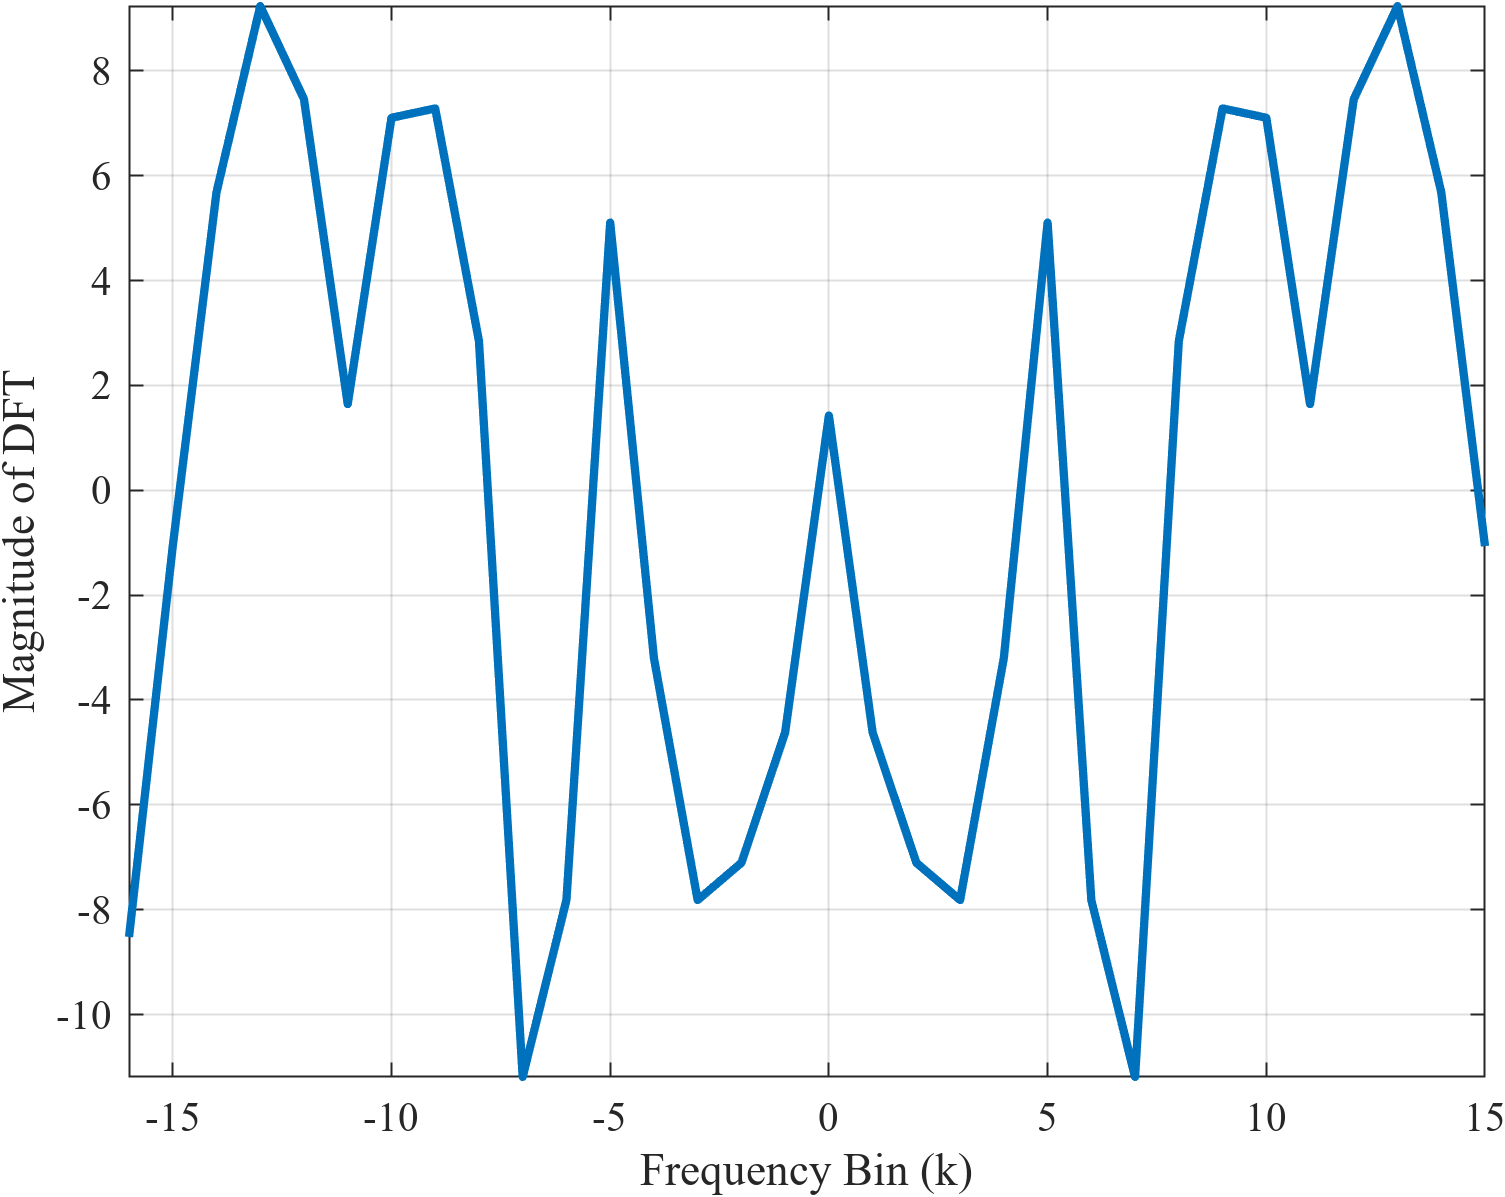
\includegraphics[width=0.8\textwidth]{F_k.png}
    \caption{32-point DFT of $f(n)$}
\end{figure}

\newpage
\section*{Problem 6: Spectral Analysis}


\newpage
\section*{Summary}
\begin{itemize}
    \item The Fourier series expansion provides a representation of the periodic signal $f(t)$ in terms of its harmonic components.
    \item The Fourier transform $F(j\omega)$ reveals the spectral content of $f(t)$, with peaks corresponding to the harmonic frequencies.
    \item The DTFT $F(e^{j\Omega})$ and the DFT provide discrete representations of the spectrum, with the DFT being limited to 32 frequency bins.
\end{itemize}

\end{document}
